
%\documentclass[mathserif]{beamer}
\documentclass[handout]{beamer}
%\usetheme{Goettingen}
%\usetheme{Warsaw}
\usetheme{Singapore}



%\usetheme{Frankfurt}
%\usetheme{Copenhagen}
%\usetheme{Szeged}
%\usetheme{Montpellier}
%\usetheme{CambridgeUS}
%\usecolortheme{}
%\setbeamercovered{transparent}
\usepackage[english, activeacute]{babel}
\usepackage[utf8]{inputenc}
\usepackage{amsmath, amssymb}
\usepackage{dsfont}
\usepackage{graphics}
\usepackage{cases}
\usepackage{graphicx}
\usepackage{pgf}
\usepackage{epsfig}
\usepackage{amssymb}
\usepackage{multirow}	
\usepackage{amstext}
\usepackage[ruled,vlined,lined]{algorithm2e}
\usepackage{amsmath}
\usepackage{epic}
\usepackage{epsfig}
\usepackage{fontenc}
\usepackage{framed,color}
\usepackage{palatino, url, multicol}
%\algsetup{indent=2em}
\newcommand{\factorial}{\ensuremath{\mbox{\sc Factorial}}}
\newcommand{\BIGOP}[1]{\mathop{\mathchoice%
{\raise-0.22em\hbox{\huge $#1$}}%
{\raise-0.05em\hbox{\Large $#1$}}{\hbox{\large $#1$}}{#1}}}
\newcommand{\bigtimes}{\BIGOP{\times}}
\vspace{-0.5cm}
\title{Natural Language Processing \\ Sequence to Sequence Models, Attention and the Transformer}
\vspace{-0.5cm}
\author[Felipe Bravo Márquez]{\footnotesize
%\author{\footnotesize  
 \textcolor[rgb]{0.00,0.00,1.00}{Felipe Bravo-Marquez}} 
  
 

\date{\today}

\begin{document}
\begin{frame}
\titlepage


\end{frame}




\begin{frame}{Language Models and Language Generation}
\begin{scriptsize}
\begin{itemize}
\item Language modeling is the task of assigning a probability to sentences in a language.
\item Example: what is the probability of seeing the sentence ``the lazy dog barked loudly''?
\item The task can be formulated as the task of predicting the probability of seing a word conditioned on previous words:
\begin{displaymath}
 P(w_i | w_1, w_2, \cdots, w_{i-1}) = \frac{P(w_1, w_2, \cdots, w_{i-1}, w_i)}{P(w_1, w_2, \cdots, w_{i-1})}  
\end{displaymath}

\end{itemize}
\end{scriptsize}
\end{frame}


\begin{frame}{Language Models and Language Generation}
\begin{scriptsize}
\begin{itemize}
\item  RNNs can be used to train language models by tying the output at time $i$ with its input at time $i + 1$ .
\item This network can be used to generate sequences of words or random sentences.
\item Generation process: predict a probability distribution over the first word conditioned on the start symbol, and draw a random word according to the predicted
distribution.

\item Then predict a probability distribution over the second word conditioned on the first, and so on, until predicting the end-of-sequence $</$s$>$ symbol.
\end{itemize}
\end{scriptsize}
\end{frame}


\begin{frame}{Language Models and Language Generation}
\begin{scriptsize}
\begin{itemize}
\item After predicting a distribution over the next output symbols $P(t_i = k | t_{1:i-1})$, a token $t_i$ is chosen and its corresponding embedding vector is fed as the input to the next step.
         \begin{figure}[h]
        	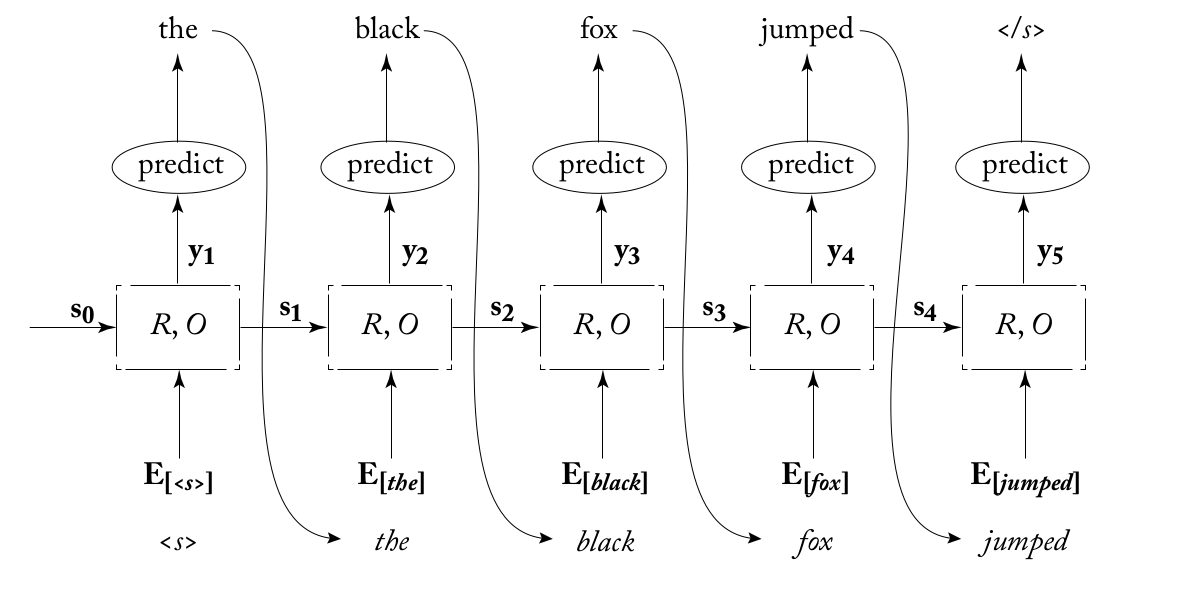
\includegraphics[scale = 0.25]{pics/generator.png}
        \end{figure}  
        
\item Teacher-forcing: during \textbf{training} the generator is fed with the ground-truth previous word even if its own prediction put a small probability mass on it. 
\item It is likely that the generator would have generated a different word at this state in \textbf{test time}.        
\end{itemize}
        
        
\end{scriptsize}
\end{frame}




\begin{frame}{Sequence to Sequence Problems}
\begin{scriptsize}
Nearly any task in NLP can be formulated as a sequence to sequence (or condionated generation) task i.e., generate output sequences from input ones. Input and output sequences can have different lengths.
\begin{itemize}
\item Machine Translation: source language to target language.
\item Summarization: long text to short text.
\item Dialogue (chatbots): previous utterances to next utterance.
\end{itemize}
\end{scriptsize}
\end{frame}



\begin{frame}{Conditioned Generation}
\begin{scriptsize}
\begin{itemize}
\item While using the RNN as a generator is a cute exercise for demonstrating its strength, the power of RNN generator is really revealed when moving to a conditioned generation or enconder-decoder framework.
\item Core idea: using two RNNs.
\item Encoder: One RNN is used to encode the source input into a vector $\overrightarrow{c}$.
\item Decoder: Another RNN is used to decode the encoder's output and generate the target output.
\item At each stage of the generation process the context vector $\overrightarrow{c}$ is concatenated to the input $\hat{t}_j$ and the concatenation is fed into the RNN.
\end{itemize}
\end{scriptsize}
\end{frame}


\begin{frame}{Encoder Decoder Framework}
         \begin{figure}[h]
        	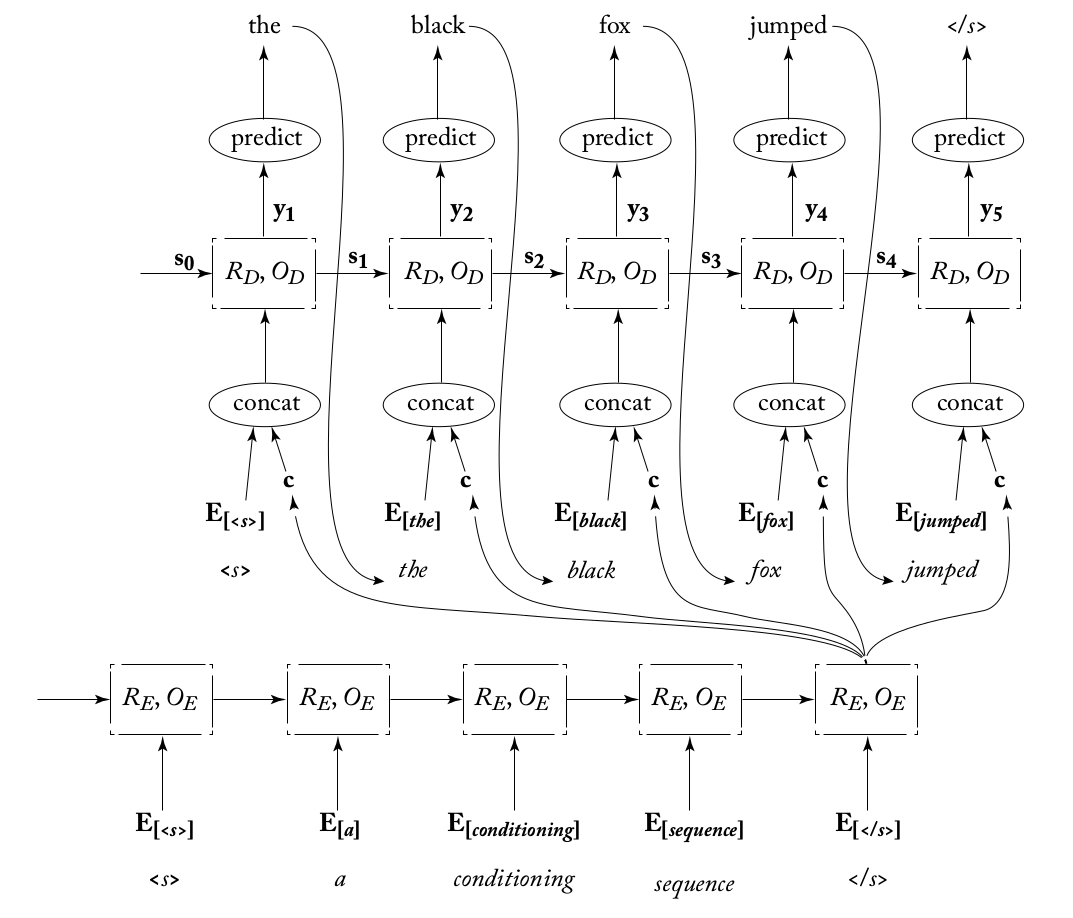
\includegraphics[scale = 0.32]{pics/seqseq.png}
        \end{figure}  
\end{frame}




\begin{frame}{Conditioned Generation}
\begin{scriptsize}
\begin{itemize}
\item This setup is useful for mapping sequences of length $n$ to sequences of length $m$.
\item The encoder summarizes the source sentence as a vector $\vec{c}$.
\item The decoder RNN is then used to predict (using a language modeling objective) the target sequence words conditioned on the previously predicted words as well as the encoded sentence $\vec{c}$.
\item The encoder and decoder RNNs are trained jointly.
\item The supervision happens only for the decoder RNN, but the gradients are propagated all the way back to the encoder RNN.
\end{itemize}
\end{scriptsize}
\end{frame}


\begin{frame}{Sequence to Sequence Training Graph}
         \begin{figure}[h]
        	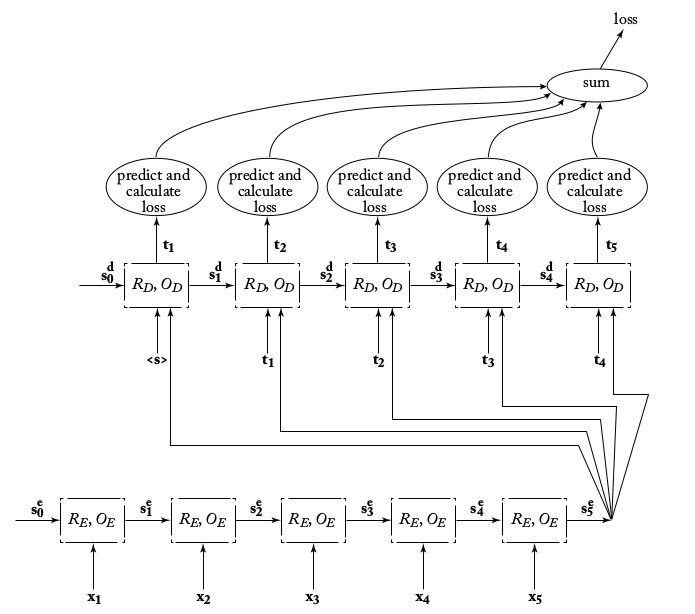
\includegraphics[scale = 0.35]{pics/seq2se2train.png}
        \end{figure}  
    
\end{frame}




\begin{frame}{Neural Machine Translation}
         \begin{figure}[h]
        	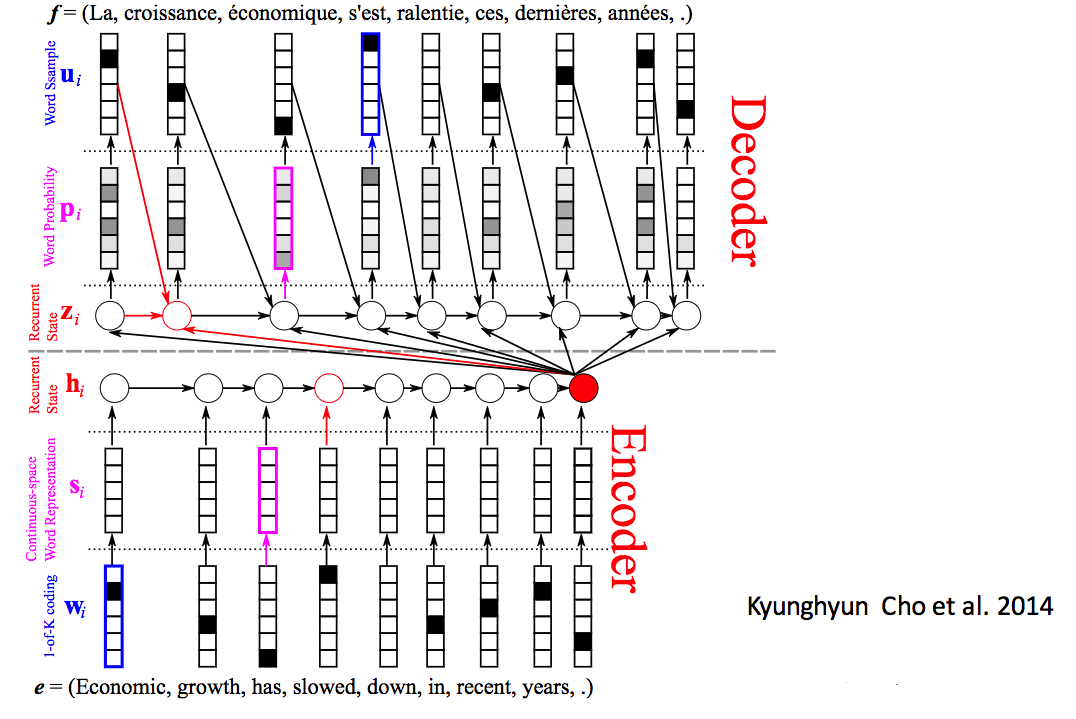
\includegraphics[scale = 0.25]{pics/mt.png}
        \end{figure}  
\end{frame}


\begin{frame}{Machine Translation BLEU progress over time}
         \begin{figure}[h]
        	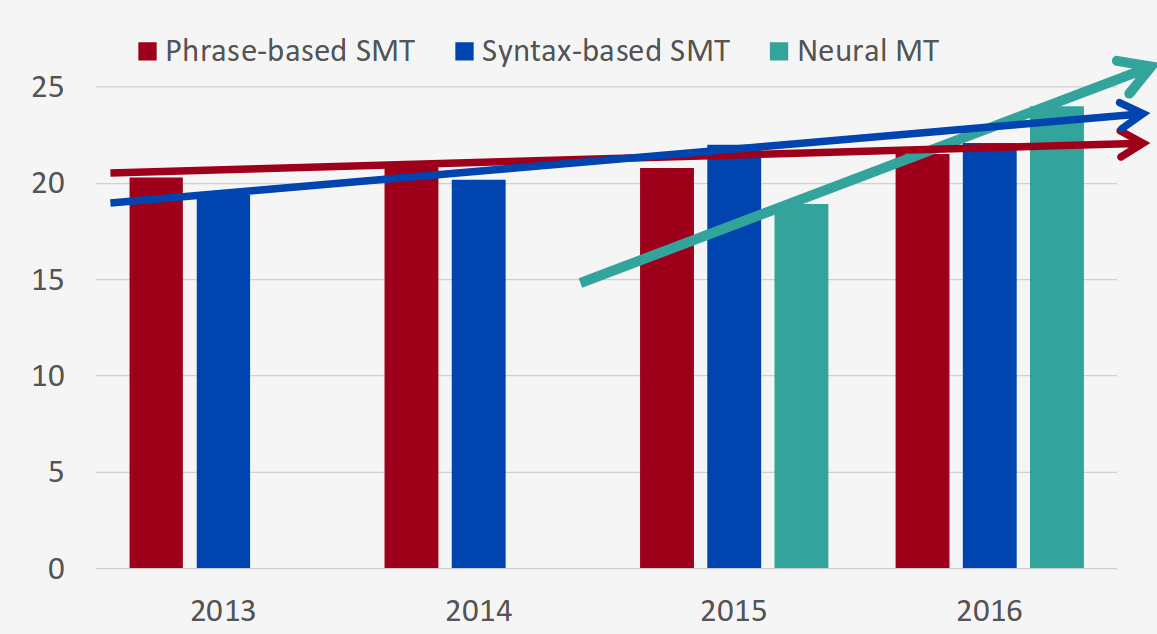
\includegraphics[scale = 0.35]{pics/nmt_progress.png}
        \end{figure}  
[Edinburgh En-De WMT]        
\footnotetext{source: \url{http://www.meta-net.eu/events/meta-forum-2016/slides/09_sennrich.pdf}}      
\end{frame}

\begin{frame}{Decoding Approaches}
\begin{scriptsize}
\begin{itemize}
\item The decoder aims to generate  the output sequence with maximal score (or maximal probability), i.e., such that $\sum_{i=1}^{n}P(\hat{t}_i | \hat{t}_{1:i-1})$ is maximized. 
\item The non-markovian nature of the RNN means that the probability function cannot be decomposed into factors that allow for exact search using standard dynamic programming.
\item Exact search: finding the optimum sequence requires evaluating every possible sequence (computationally prohibitive).
\item Thus, it only makes sense to solving the optimization problem above approximately.
\item Greedy search: choose the highest scoring prediction (word) at each step.
\item This may result in sub-optimal overall probability leading to
prefixes that are followed by low-probability events.

\end{itemize}
        
        
\end{scriptsize}
\end{frame}


\begin{frame}{Greedy Search}
        
         \begin{figure}[h]
        	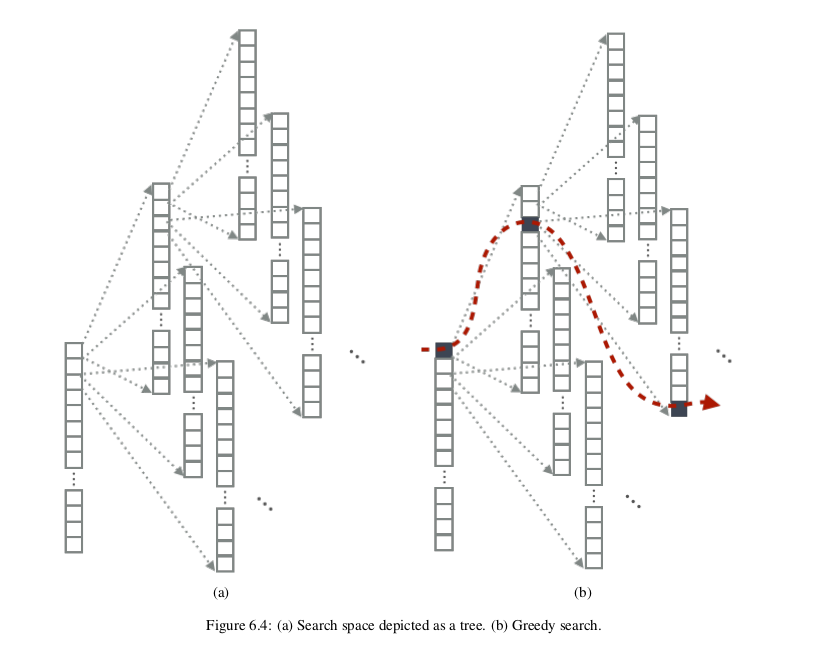
\includegraphics[scale = 0.3]{pics/greedysearch.png}
        \end{figure}        
        
        
        
\footnotetext{Source: \cite{cho2015natural}}
        
\end{frame}



\begin{frame}{Beam Search}
\begin{scriptsize}
\begin{itemize}
\item Beam search interpolates between the exact search and the greedy search by changing the size $K$ of hypotheses maintained throughout the search procedure \cite{cho2015natural}.
\item The Beam search algorithm works in stages.
\item  We first pick the $K$ starting words with the highest probability 
\item At each step, each candidate sequence is expanded with all possible next steps. 
\item Each candidate step is scored. 
\item The $K$ sequences with the most likely probabilities are retained and all other candidates are pruned. 
\item The search process can halt for each candidate separately either by reaching a maximum length, by reaching an end-of-sequence token, or by reaching a threshold likelihood.
\item The sentence with the highest overall probability is selected.
\end{itemize}
        
\footnotetext{More info at: \url{https://machinelearningmastery.com/beam-search-decoder-natural-language-processing/}}        
\end{scriptsize}
\end{frame}





\begin{frame}{Conditioned Generation with Attention}
\begin{scriptsize}
\begin{itemize}
\item In the encoder-decoder networks the input sentence is encoded into a single vector, which is then used as a conditioning context for an RNN-generator. 
\item This architectures forces the encoded vector $\vec{c}$ to contain all the information required for generation.
\item It doesn't work well for long sentences!
\item It also requires the generator to be able to extract this information from the fixed-length vector.
\item ``You can't cram the meaning of a whole \%\&!\$\# sentence into a single \$\&!\#* vector!'' -Raymond Mooney
\item This architecture can be can be substantially improved (in many cases it) by the addition of an attention mechanism.
\item The attention mechanism attempts to solve this problem by allowing the decoder to “look back” at the encoder’s hidden states based on its current state. 
\end{itemize}
\end{scriptsize}
\end{frame}



\begin{frame}{Conditioned Generation with Attention}
\begin{scriptsize}
\begin{itemize}
\item The input sentence (a length $n$ input sequence $\vec{x}_{1:n}$) is encoded using a biRNN as a sequence of vectors $\vec{c}_{1:n}$.  
\item The decoder uses a soft attention mechanism in order to decide on which parts of the encoding input it should focus. 
\item At each stage $j$ the decoder sees a weighted average of the vectors $\vec{c}_{1:n}$ , where the attention weights ($\vec{\alpha}^j$) are chosen by the attention mechanism.
\begin{displaymath}
\vec{c}^j = \sum_{i=1}^{n} \vec{\alpha}_{[i]}^{j}\cdot \vec{c}_i 
\end{displaymath}
\item The elemements of $\vec{\alpha}^j$ are all positive and sum to one.



\end{itemize}
\end{scriptsize}
\end{frame}





\begin{frame}{Conditioned Generation with Attention}
\begin{scriptsize}
\begin{itemize}
\item Unnormalized attention weights ($\bar{\alpha}_{[i]}^j$)  are produced taking into account the decoder state at time $j$ ($\vec{s}_j$) and each of the vectors $\vec{c}_i$.
\item They can be obtained in various ways, basically any differentiable function returning a scalar out of two vectors $\vec{s}_j$ and  $\vec{c}_i$ could be employed. 
\item The simplest approach is a dot product:  $\bar{\alpha}_{[i]}^j = \vec{s}_j \cdot \vec{c}_i$. 
\item The one we will use in these slides is Additive attention, which uses a Multilayer Perceptron: $\bar{\alpha}_{[i]}^j = MLP^{att}([\vec{s}_j;\vec{c}_i]) = \vec{v} \cdot \operatorname{tanh}([\vec{s}_j;\vec{c}_i]U +\vec{b})$

\end{itemize}
\end{scriptsize}
\end{frame}


\begin{frame}{Conditioned Generation with Attention}
\begin{scriptsize}
\begin{itemize}
\item These unnormalized weights are then normalized into a probability distribution using the softmax function.

\begin{figure}[h]
        	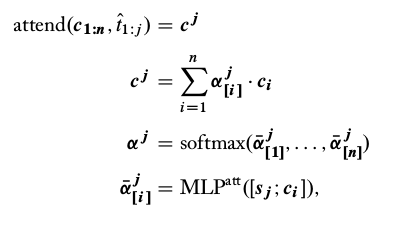
\includegraphics[scale = 0.35]{pics/atten_formula.png}
        \end{figure}  

        
                

\item The encoder, decoder, and attention mechanism are all trained jointly in order to play well with each other.


\end{itemize}
\end{scriptsize}
\end{frame}





\begin{frame}{Attention}
         \begin{figure}[h]
        	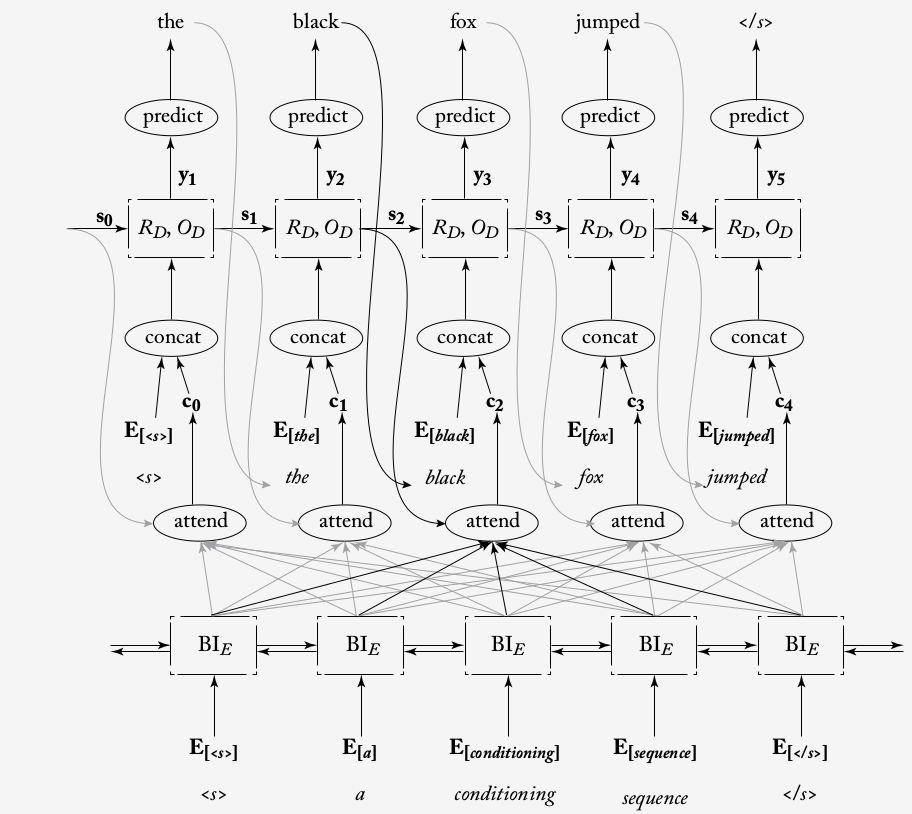
\includegraphics[scale = 0.35]{pics/encdecattention.png}
        \end{figure}  
\end{frame}



\begin{frame}{Conditioned Generation with Attention}
\begin{scriptsize}
The entire sequence-to-sequence generation with attention is given by:

\begin{figure}[h]
        	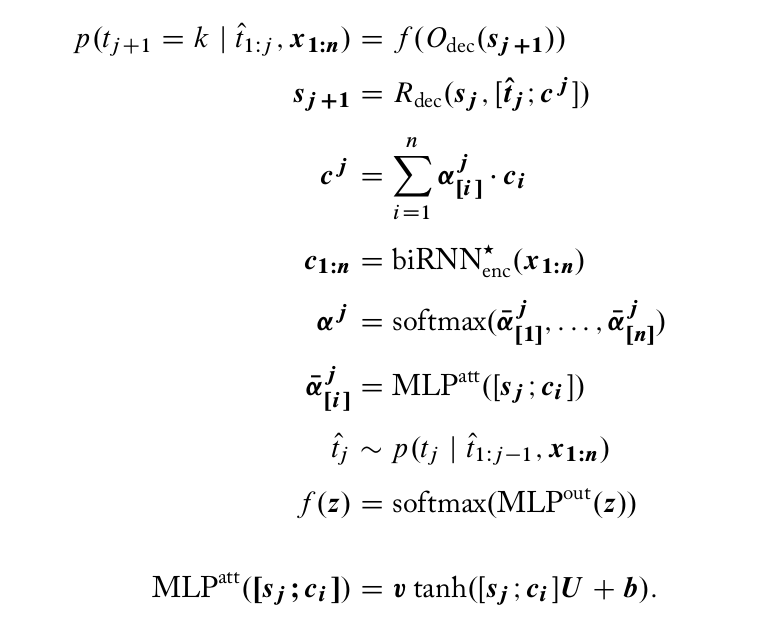
\includegraphics[scale = 0.3]{pics/attentionformula.png}
        \end{figure}  

        
                
\end{scriptsize}
\end{frame}



\begin{frame}{Conditioned Generation with Attention}
\begin{scriptsize}
\begin{itemize}
\item Why use the biRNN encoder to translate the conditioning sequence $\vec{x}_{1:n}$  into the context vectors $\vec{c}_{1:n}$?
\item Why we just don't attend directly on the inputs (word embeddings) $MLP^{att}([\vec{s}_j;\vec{x}_i])$?
\item We could, but we get important benefits from the encoding process.
\item First, the biRNN vectors $\vec{c}_i$ represent the items $\vec{x}_i$ in their sentential context.
\item Sentential context: a window focused around the input item $\vec{x}_i$ and not the item itself.
\item Second, by having a trainable encoding component that is trained jointly with the decoder, the encoder and decoder evolve together.
\item Hence, the network can learn to encode relevant properties of the input that are useful for decoding, and that may not be present at the source sequence $\vec{x}_{1:n}$ directly.
\end{itemize}
\end{scriptsize}
\end{frame}


\begin{frame}{Attention and Word Alignments}
\begin{scriptsize}
\begin{itemize}
\item In the context of machine translation, one can think of $MLP^{att}$ as computing a soft alignment between the current decoder state $\vec{s}_j$ (capturing the recently produced foreign words) and each of the source sentence components $\vec{c}_i$.


\end{itemize}


         \begin{figure}[h]
        	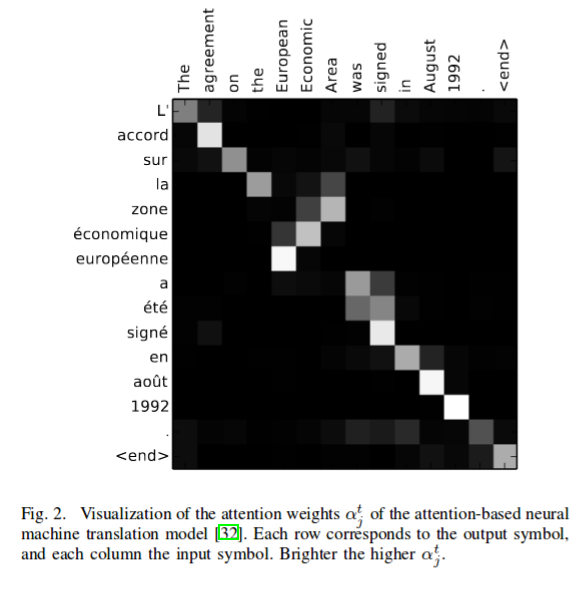
\includegraphics[scale = 0.28]{pics/attention-alignment.png}
        	\caption{Source: \cite{cho2015describing}}
        \end{figure}  


\end{scriptsize}
\end{frame}



\begin{frame}{Other types of Attention}
\begin{scriptsize}

       \begin{figure}[h]
        	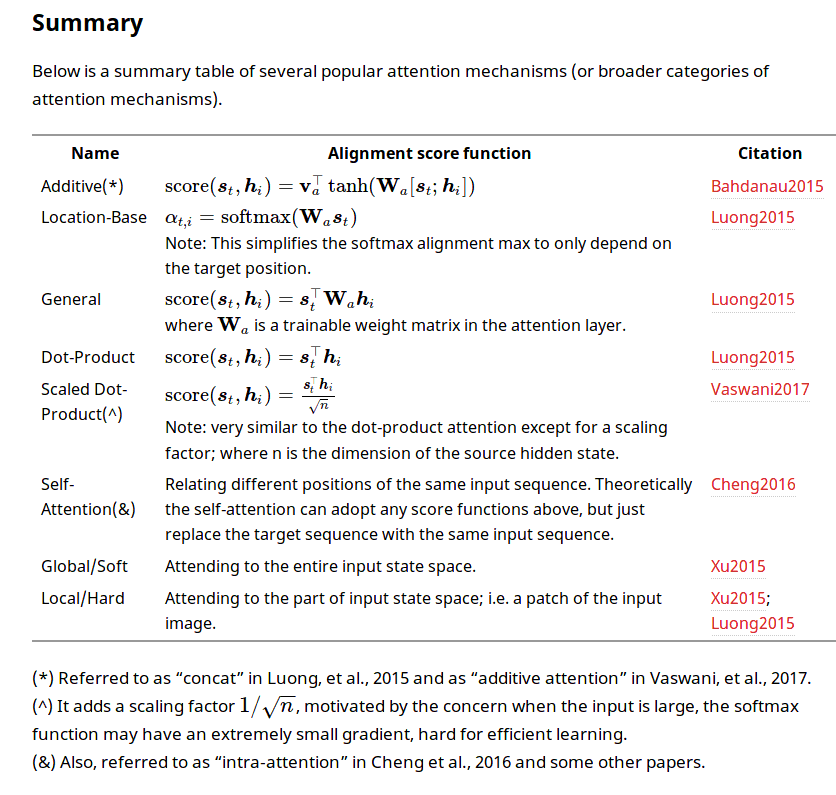
\includegraphics[scale = 0.32]{pics/types_of_attention.png}
        	\caption{Source: \url{https://lilianweng.github.io/lil-log/2018/06/24/attention-attention.html}}
        \end{figure}  


\end{scriptsize}
\end{frame}

\begin{frame}{What's Wrong with RNNs?}
\begin{scriptsize}
\begin{itemize}
\item Given what we just learned above, it would seem like attention solves all the problems with RNNs and encoder-decoder architectures\footnote{The following material is based on: \url{http://mlexplained.com/2017/12/29/attention-is-all-you-need-explained/}}.

\item There are a few shortcomings of RNNs that another architecture called the \textbf{Transformer} tries to address.

\item The Transformer discards the recursive component of the Encoder-Decoder architecture and purely relies on attention mechanisms \cite{vaswani2017attention}.

\item When we process a sequence using RNNs, each hidden state depends on the previous hidden state. 

\item This becomes a major pain point on GPUs: GPUs have a lot of computational capability and they hate having to wait for data to become available.

\item Even with technologies like CuDNN, RNNs are painfully inefficient and slow on the GPU.


\end{itemize}
\end{scriptsize}
\end{frame}

\begin{frame}{Dependencies in neural machine translations}
\begin{scriptsize}
In essence, there are three kinds of dependencies in neural machine translations: 
\begin{enumerate}
\item Dependencies between the input and output tokens.

\item Dependencies between the input tokens themselves.

\item Dependencies between the output tokens themselves.
\end{enumerate}


The traditional attention mechanism largely solved the first dependency by giving the decoder access to the entire input sequence. The second and third depedencies were addressed by the RNNs.

\end{scriptsize}

\end{frame}


\begin{frame}{The Transformer}
\begin{scriptsize}
\begin{itemize}
 \item The novel idea of the Transformer is to extend this mechanism to the processing input and output sentences as well.
 \item The RNN processes input sequences sequentialy. 
 \item The Transformer, on the other hand, allows the encoder and decoder to see the entire input sequence all at once.
 \item This is done using attention.
\end{itemize}



\end{scriptsize}

\end{frame}




\begin{frame}{The Key Component: Multi-Head Attention}
\begin{scriptsize}
\begin{itemize}
 \item The attention mechanism in the Transformer is interpreted as a way of computing the relevance of a set of \textbf{values} (information) based on some \textbf{keys} and \textbf{queries}. 
 
 \item The attention mechanism is used as a way for the model to \textbf{focus on relevant information} based on what it is currently processing.
 
 \item In the RNN encoder-decoder architecture with attention:
 

 \begin{enumerate}
  \begin{scriptsize}
 \item Attention weights were the relevance of the encoder hidden states (values) in processing the decoder state (query).
 
 \item These values were calculated based on the encoder hidden states (keys) and the decoder hidden state (query).
 \end{scriptsize}

 \end{enumerate}

 
\end{itemize}



\end{scriptsize}

\end{frame}


\begin{frame}{The Key Component: Multi-Head Attention}

    \begin{figure}[h]
        	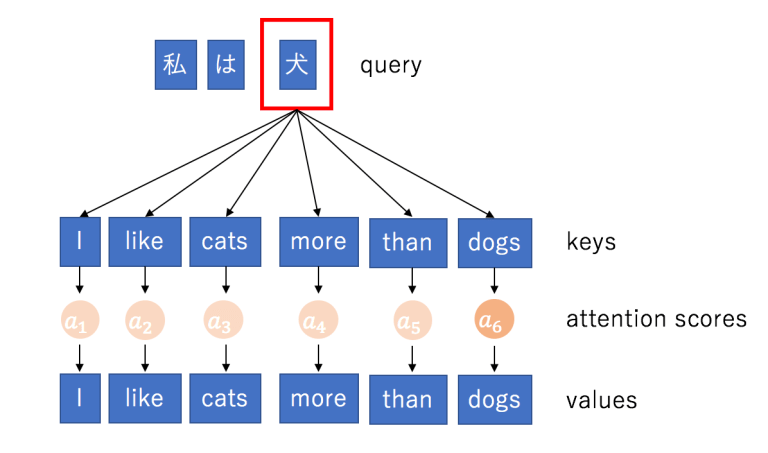
\includegraphics[scale = 0.28]{pics/attention_concept.png}
        	\caption{In this example, the query is the word being decoded (which means dog) and both the keys and values are the source sentence. The attention score represents the relevance, and in this case is large for the word “dog” and small for others.}
        \end{figure}  

\end{frame}




\begin{frame}{The Key Component: Multi-Head Attention}
\begin{scriptsize}
\begin{itemize}
 \item When we think of attention this way, we can see that the keys, values, and queries could be anything. 
 \item They could even be the same. 
 \item For instance, both values and queries could be input embeddings (self attention). 
 
 \item If we only computed a single attention weighted sum of the values, it would be difficult to capture various different aspects of the input.
 

\end{itemize}

\end{scriptsize}

\end{frame}



\begin{frame}{The Key Component: Multi-Head Attention}
\begin{scriptsize}
\begin{itemize}
 \item For instance, in the sentence ``I like cats more than dogs'', you might want to capture the fact that the sentence compares two entities, while also retaining the actual entities being compared. 
 
 \item To solve this problem the Transformer uses the Multi-Head Attention block. 
 
 \item This block computes multiple attention weighted sums instead of a single attention pass over the values.
 
 \item Hence the name ``Multi-Head'' Attention.
 
 
 
\end{itemize}

\end{scriptsize}

\end{frame}


\begin{frame}{The Key Component: Multi-Head Attention}
\begin{scriptsize}
\begin{itemize}
 \item To learn diverse representations, the Multi-Head Attention applies different linear transformations to the values, keys, and queries for each “head” of attention.
 
 
     \begin{figure}[h]
        	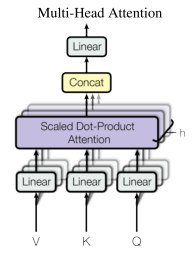
\includegraphics[scale = 0.48]{pics/multi_head_attention.png}
        \end{figure}  
 

\end{itemize}

\end{scriptsize}

\end{frame}



\begin{frame}{The Key Component: Multi-Head Attention}
\begin{scriptsize}
\begin{itemize}

 \item A single attention applies a unique linear transformation to its input queries, keys, and values.
 
 \item Then computes the attention score between each query and key.
 
 \item The attention score is used to weight the values and sum them up.


\item The Multi-Head Attention block just applies multiple blocks in parallel, concatenates their outputs, then applies one single linear transformation. 
 
\end{itemize}

\end{scriptsize}

\end{frame}


\begin{frame}{Scaled Dot Product Attention}
\begin{scriptsize}
\begin{itemize}

 \item  Transformer uses a particular form of attention called the “Scaled Dot-Product Attention”:
 \begin{displaymath}
  \text{Attention}(Q,K,V) = \text{softmax}\left(\frac{QK^T}{\sqrt{d_k}}\right)V
 \end{displaymath}

 \item where $Q$ is the matrix of queries packed together and $K$ and $V$ are the matrices of keys and values packed together. 
 
 \item $d_k$ represents the dimensionality of the queries and keys.
 
  \item The normalization over $\sqrt{d_k}$ is used to rescale the dot products between queries and keys (dot products tend to grow with the dimensionality).
 
\end{itemize}

\end{scriptsize}

\end{frame}


\begin{frame}{The Transformer}

     \begin{figure}[h]
        	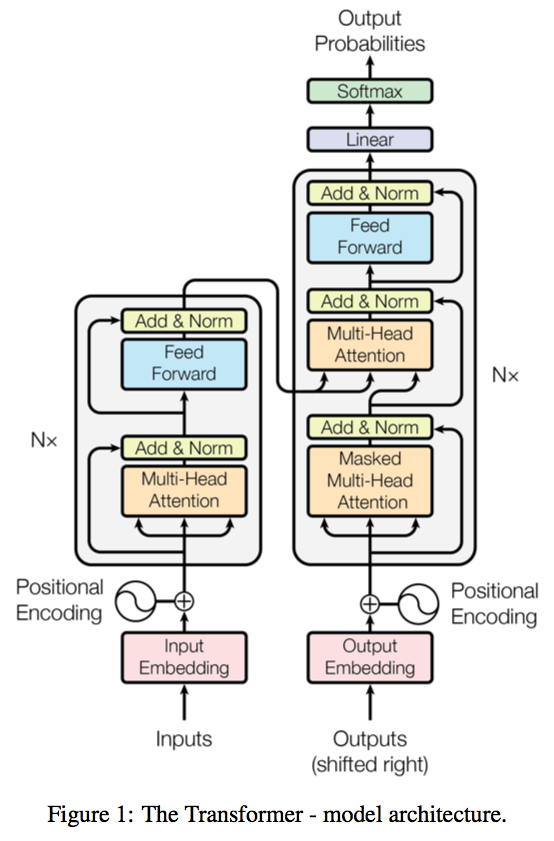
\includegraphics[scale = 0.29]{pics/transformer.png}
        \end{figure}  


\end{frame}


\begin{frame}{The Transformer}
\begin{scriptsize}
\begin{itemize}

 \item  The Transformer still uses the basic encoder-decoder design of RNN neural machine translation systems.
 
 \item The left-hand side is the encoder, and the right-hand side is the decoder. 
 
 \item The initial inputs to the encoder are the embeddings of the input sequence.
 \item The initial inputs to the decoder are the embeddings of the outputs up to that point. 
 
 \item The encoder and decoder are composed of $N$ blocks (where $N = 6$ for both networks).
 
 \item These blocks are composed of smaller blocks as well. 
 
 \item Let's look at each block in further detail.
 
\end{itemize}

\end{scriptsize}

\end{frame}



\begin{frame}{The Encoder}
\begin{scriptsize}
\begin{itemize}

\item The encoder contains self-attention layers. 

\item In a self-attention layer all of the keys, values and queries come from the same place, in this case, the output of the previous layer in the encoder. 

\item Each position in the encoder can attend to all positions in the previous layer of the encoder.

 \item  The encoder is composed of two blocks (which we will call sub-layers to distinguish from the $N$ blocks composing the encoder and decoder).
\item  One is the Multi-Head Attention sub-layer over the inputs, mentioned above. 
\item The other is a simple feed-forward network. 

\end{itemize}

\end{scriptsize}

\end{frame}


\begin{frame}{The Encoder}
\begin{scriptsize}
\begin{itemize}

\item Between each sub-layer, there is a residual connection followed by a layer normalization. 

\item A residual connection is basically just taking the input and adding it to the output of the sub-network, and is a way of making training deep networks easier. 

\item Layer normalization is a normalization method in deep learning that is similar to batch normalization.
 
\end{itemize}

\end{scriptsize}

\end{frame}



\begin{frame}{The Encoder}

     \begin{figure}[h]
        	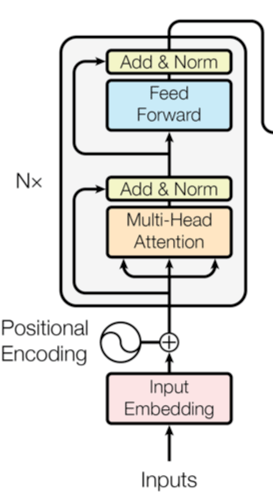
\includegraphics[scale = 0.39]{pics/transformerencoder.png}
        \end{figure}  


\end{frame}

\begin{frame}{The Encoder}
\begin{scriptsize}
\begin{itemize}

 \item  What each encoder block is doing is actually just a bunch of matrix multiplications followed by a couple of element-wise transformations.
 
 \item This is why the Transformer is so fast: everything is just parallelizable matrix multiplications.
 
 \item The point is that by stacking these transformations on top of each other, we can create a very powerful network. 
 
 \item The core of this is the attention mechanism which modifies and attends over a wide range of information.
 
\end{itemize}

\end{scriptsize}

\end{frame}



\begin{frame}{The Decoder}
\begin{scriptsize}
\begin{itemize}



\item The decoder has ``encoder-decoder attention'' layers in which the queries come from the previous decoder layer,and the memory keys and values come from the output of the encoder.

\item This allows every position in the decoder to attend over all positions in the input sequence.

\item This mimics the typical encoder-decoder attention mechanisms in sequence-to-sequence models.

\item Self-attention layers in the decoder allow each position in the decoder to attend to all positions in the decoder up to and including that position.

 \item This plays a similar role to the decoder hidden state in RNN machine translation architectures.


 
\end{itemize}

\end{scriptsize}

\end{frame}





\begin{frame}{The Decoder}
\begin{scriptsize}
\begin{itemize}
 \item When we train the Transformer, we want to process all the sentences at the same time. 
 
 \item When we do this, if we give the decoder access to the entire target sentence, the model can just repeat the target sentence (in other words, it doesn't need to learn anything).
 
 \item To prevent this from happening, the decoder masks the ``future'' tokens when decoding a certain word.

  \item The masking is done by setting to $- \infty$ all values in the input of the softmax which correspond to illegal connections.
 \item This is why ``multi-head attention blocks'' in the decoder are referred to as ``masked'': the inputs to the decoder from future time-steps ared masked.

\end{itemize}

\end{scriptsize}

\end{frame}


\begin{frame}{The Decoder}

     \begin{figure}[h]
        	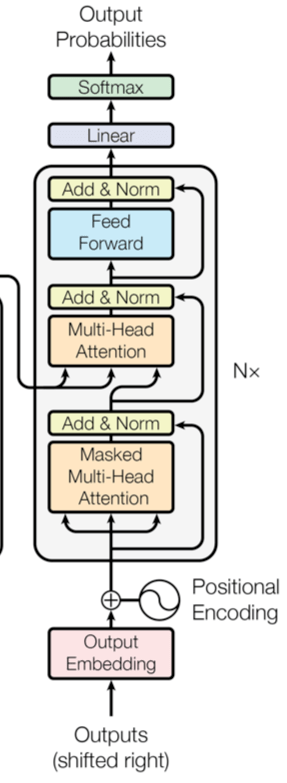
\includegraphics[scale = 0.29]{pics/transformerdecoder.png}
        \end{figure}  


\end{frame}



\begin{frame}{Positional Encodings}
\begin{scriptsize}
\begin{itemize}

 \item  Unlike recurrent networks, the multi-head attention network cannot naturally make use of the position of the words in the input sequence.
 
 \item Without positional encodings, the output of the multi-head attention network would be the same for the sentences ``I like cats more than dogs'' and ``I like dogs more than cats''.
 
 \item Positional encodings explicitly encode the relative/absolute positions of the inputs as vectors and are then added to the input embeddings.

\end{itemize}

\end{scriptsize}


\end{frame}

\begin{frame}{Positional Encodings}
\begin{scriptsize}
\begin{itemize}

 \item The paper uses the following equation to compute the positional encodings: \\
 $PE(pos,2i) = \sin(pos/10000^{2i/d_{model}})$ 
  $PE(pos,2i+1) = \cos(pos/10000^{2i/d_{model}})$
 
\item Where $pos$ represents the position, and $i$ is the dimension.

\item Basically, each dimension of the positional encoding is a wave with a different frequency. 


\end{itemize}

\end{scriptsize}


\end{frame}


\begin{frame}{Conclusions}
\begin{scriptsize}
\begin{itemize}

 \item The Transformer achieves better BLUE scores than previous state-of-the-art models for English-to-German translation and English-to-French translation at a fraction of the training cost.

      \begin{figure}[h]
        	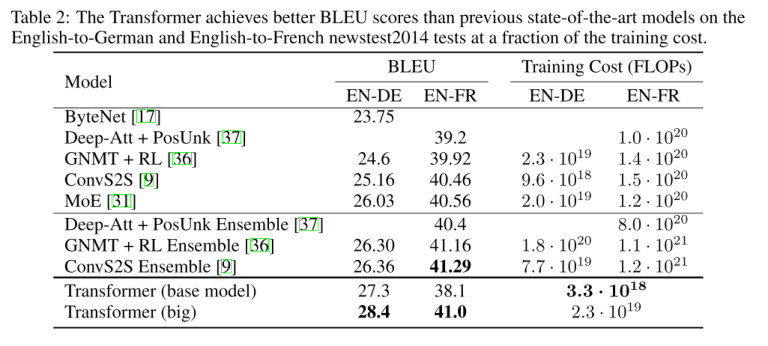
\includegraphics[scale = 0.29]{pics/transformerresults.png}
        \end{figure}  

\item The Transformer is a powerful and efficient alternative to recurrent neural networks to model dependencies using only attention mechanisms.

 
\end{itemize}

\end{scriptsize}


\end{frame}

\begin{frame}
\frametitle{Questions?}
%\vspace{1.5cm}
\begin{center}\LARGE Thanks for your Attention!\\ \end{center}



\end{frame}

\begin{frame}[allowframebreaks]\scriptsize
\frametitle{References}
\bibliography{bio}
\bibliographystyle{apalike}
%\bibliographystyle{flexbib}
\end{frame}  


%%%%%%%%%%%%%%%%%%%%%%%%%%%

\end{document}
